\chapter{Methodology}
\section{Object Detection Architectures and Backbones}
\label{sec:arch_and_backbones}
The core of our lung nodule detection pipeline is built upon a robust and well-established object detection framework. For this research, experiments will be conducted on the architectures discussed in the previous chapter: Faster R-CNN and RetinaNet.

While these architectures defines the overall detection process, the quality of the features extracted from the input image is can impact its success. This feature extraction is performed by a deep convolutional neural network, commonly referred to as the backbone. The choice of backbone directly influences the model's performance, computational complexity, and memory footprint. A central component of our methodology is therefore to systematically evaluate the impact of different backbone architectures on the lung nodule detection task.

To investigate the trade-off between model performance and computational efficiency, we conducted experiments with three distinct backbone architectures, each representing a different design philosophy:

\begin{itemize}
    \item \textbf{ResNet50:} A canonical and widely adopted architecture, ResNet50 serves as a robust and powerful baseline. Its use of residual connections allows for the effective training of very deep networks, making it a standard choice for a vast range of computer vision tasks. With 25.5 million parameters, it represents a high-performance, but computationally intensive, option.

    \item \textbf{MobileNetV2:} Designed specifically for efficiency and deployment on resource constrained devices, MobileNetV2 is a lightweight architecture with only 5.4 million parameters. It utilizes inverted residual blocks and linear bottlenecks to achieve a favorable balance between accuracy and computational cost, making it an ideal candidate for exploring the feasibility of more accessible clinical tools.

    \item \textbf{EfficientNetV2-S:} This model represents a modern approach to network design, seeking to optimally balance accuracy, training speed, and parameter efficiency. By systematically scaling network depth, width, and resolution, and employing novel architectural blocks, EfficientNetV2-S (with 21.4 million parameters) offers performance competitive with larger models while maintaining a smaller computational footprint.
\end{itemize}

In all experiments, each backbone was initialized with weights pre-trained on the ImageNet1k dataset. This transfer learning approach is a standard practice that leverages the rich, hierarchical features learned from a large-scale, general-purpose dataset to significantly improve performance and reduce training time on smaller, specialized datasets such as the one used in this study. 

\subsection{Loss functions}
\label{sec:loss_functions}
A central metric for bounding box quality is the \textit{Intersection over Union} (IoU):
$$
\mathrm{IoU}(b, b^\ast) = \frac{\mathrm{area}(b \cap b^\ast)}{\mathrm{area}(b \cup b^\ast)},
$$
which measures the degree of spatial overlap between a predicted box $b$ and a ground-truth box $b^\ast$.
Variants such as Generalized IoU (GIoU), Distance IoU (DIoU), and Complete IoU (CIoU) incorporate additional geometric terms to improve optimization stability, particularly when boxes do not overlap \cite{rezatofighi2019giou,zheng2019diou, zheng2021ciou}.


Bounding box regression is also commonly evaluated in coordinate space using Minkowski distances.
The general $p$-norm between two vectors $u,v \in \mathbb{R}^n$ is defined as:
$$
\| u - v \|_p = \left( \sum_{j=1}^n |u_j - v_j|^p \right)^{\frac{1}{p}}.
$$
Special cases include the Manhattan distance ($L_1$ norm, $p=1$):
$$
\| u - v \|_1 = \sum_{j=1}^n |u_j - v_j|,
$$
and the Euclidean distance ($L_2$ norm, $p=2$):
$$
\| u - v \|_2 = \sqrt{\sum_{j=1}^n (u_j - v_j)^2}.
$$

In practice, modern detectors often adopt the Smooth-$L_1$ loss \cite{girshick2015fastrcnn} for bounding box regression, which combines the robustness of $L_1$ for large errors with the stability of $L_2$ for small errors:
$$
\mathrm{SmoothL1}(x) =
\begin{cases}
0.5\,x^2, & \text{if } |x| < 1, \\
|x| - 0.5, & \text{otherwise}.
\end{cases}
$$
This formulation reduces sensitivity to outliers while maintaining differentiability at the origin, making it suitable for gradient-based optimization.

As for the classification component, Faster R-CNN employs the standard cross-entropy loss for binary classification tasks, while RetinaNet utilizes the Focal Loss \cite{lin2018focalloss} to address class imbalance by down-weighting easy negatives and focusing training on hard examples.

\section{Data Preprocessing}

\subsection{Train-time Augmentations}
\label{sec:augmentation}
To further enhance the robustness of our models and improve their generalization capabilities, we apply a series of data augmentations during training. These augmentations include random rotations, flips, and intensity variations, which help to simulate the variability encountered in real-world clinical settings. By exposing the model to a diverse set of augmented images, we aim to reduce overfitting and improve the model's ability to generalize to unseen data. These augmentations are applied on-the-fly during training, ensuring that the model sees a different version of the data in each epoch.

The specific augmentations applied are as follows:
\begin{itemize}
    \item \textbf{Horizonal Flips}: Each image has a 50\% chance of being flipped horizontally. This augmentation helps the model learn invariance to left-right orientation, which is particularly relevant in medical imaging where anatomical structures can appear in various orientations.
    \item \textbf{Shift, Scale and Rotate}: Each image has a 50\% change of being randomly shifted (up to 5\% of image dimensions), scaled (between 0.9 and 1.1 times the original size), and rotated (up to 15 degrees). These transformations simulate variations in patient positioning and imaging angles, enhancing the model's ability to recognize nodules under different conditions.
    \item \textbf{Random Brightness and Contrast}: Each image has a 50\% chance of having its brightness and contrast randomly adjusted. Brightness is modified by a factor between -0.1 and +0.1, while contrast is adjusted by a factor between 0.9 and 1.1. This augmentation accounts for differences in imaging protocols and equipment, helping the model to generalize across varying image qualities.
    \item \textbf{CLAHE (Contrast Limited Adaptive Histogram Equalization)}: \\Each image has a 50\% chance of being processed with CLAHE. This technique enhances local contrast and improves the visibility of structures in areas that are too dark or too bright, which is particularly useful in medical images where subtle features can be critical for diagnosis \cite{mishra2021clahe}.
\end{itemize}


\subsection{Slice Selection Algorithms}
\label{sec:dataset_pruning}
% Explain the need for slice selection algorithms in this 2D setting, as some might not contain relevan information (nodule mass). explain the statistical approach, the sliding window approach and finally the simple thresholding approach.
A preliminary analysis revealed that the model's performance on the Duke Lung Cancer Screening (DLCS) dataset was significantly lower than on the National Lung Screening Trial (NLST) dataset. This discrepancy is attributed not only to the model's limitations but also to the inherent challenges of the DLCS data itself, primarily the smaller and more variable size of nodules and the nature of the volumetric annotations.

After a brief analysis became apparent that a significant portion of the extracted 2D slices did not contain any nodules or relevant anatomical structures. This is particularly true for the upper and lower regions of the extracted nodules, where the section of the cancerous tissue is minimal or non-existent (see Figure~\ref{fig:non-visible-nodule}).

\begin{figure}[h]
    \centering
    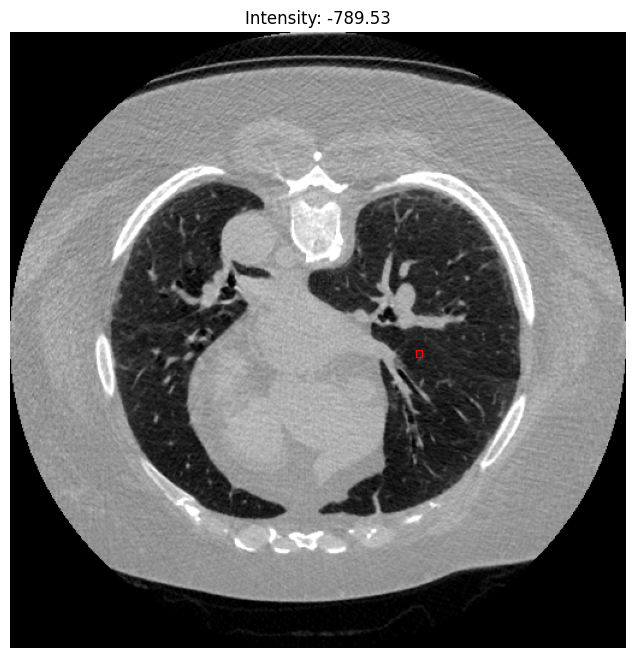
\includegraphics[width=0.6\linewidth]{images/non-visible-nodule-1.png}
    \caption{Example of a slice with an annotated nodule (at the indicated depth) that does not contain any visible tissue from the nodule itself. At the top the mean intensity expressed in Hounsfield Units (HU) of the area within the annotation. }
    \label{fig:non-visible-nodule}
\end{figure}

The strategy of extracting every 2D slice from a 3D volumetric bounding box is susceptible to annotation inaccuracies. Volumetric annotations are rarely perfect, often including slices at the superior and inferior extremes where the nodule is barely visible or entirely absent. Training the model on these "empty" or noisy slices can introduce a significant amount of label noise, potentially degrading its performance by forcing it to learn from irrelevant or misleading examples.

To mitigate this, a dataset pruning strategy was developed to selectively remove these low-information slices. Several approaches were investigated to identify and remove them in a principled manner.

\subsubsection{Exploration of Pruning Strategies}
The core assumption behind our pruning is that slices containing predominantly healthy lung tissue or air will have a significantly lower average Hounsfield Unit (HU) intensity within the annotated bounding box compared to slices containing dense tumorous tissue. Based on this, the following strategies were explored:

\paragraph{Statistical Outlier Detection:} This initial approach, detailed in Algorithm \ref{alg:stat-pruning}, involved calculating the median ($\tilde{m}$) and Interquartile Range (IQR) of the mean bounding box intensities for all slices belonging to a single nodule. Slices with intensities considered to be low-end outliers were removed. However, this method proved to be overly aggressive, eliminating a substantial number of slices (~50\% of the dataset), including many that contained valuable information.

\begin{algorithm}[H]
    \caption{Strategy 1: Statistical Pruning}
    \label{alg:stat-pruning}
    \DontPrintSemicolon
    \SetAlgoLined
    \setstretch{1.2}

    \SetKwInOut{Input}{Input}
    \Input{
        SlicesForNodule: a list of (slice, mean\_intensity) pairs for one nodule\;
        $\alpha$: an adjustment factor (e.g., 1.5)
    }
    \SetKwData{keptSlices}{kept\_slices}
    \SetKwData{meanIntensities}{mean\_intensities}
    
    \BlankLine
    
    $\meanIntensities \gets$ [s.mean\_intensity for s in SlicesForNodule]\;
    Q1 $\gets$ FirstQuartile($\meanIntensities$)\;
    IQR $\gets$ InterquartileRange($\meanIntensities$)\;
    threshold $\gets$ Q1 - ($\alpha \times$ IQR)\;
    
    \BlankLine
    $\keptSlices \gets \{\}$\;
    \ForAll(){(slice, intensity) \textup{in} SlicesForNodule}{
        \If{intensity $\geq$ threshold}{
            $\keptSlices$.add(slice)\;
        }
    }
    \Return{$\keptSlices$}\;
\end{algorithm}


This approach, although being statistically sound, it tries to estimate properties of the mean intensity distribution, namely median and IQR, of each sample given a very limited number of slices for each nodule. This limitation often leads to an overly aggressive pruning, as the statistical estimates may not accurately reflect the true distribution of intensities.
It may also happen that if a given annotation is particularly noisy, shallow or generally mostly uninformative, the statistical properties of the mean intensity distribution may be skewed, leading to the opposite effect, removing informative slices as they might be detected as outliers of the distribution.

\paragraph{Sliding Window Approach:} To incorporate spatial locality, a sliding window of size $K$ was moved along the z-axis of each nodule (slices sorted by height). The window position that maximized the cumulative mean intensity was considered to contain the core of the nodule, as shown in Algorithm \ref{alg:sliding-window-pruning}. While this produced more coherent results, it was sensitive to the choice of $K$ and the full strategy (testing all possible values of $K$ and using an elbow method to choose the best one) proved overly complex.

\begin{algorithm}[H]
    \caption{Strategy 2: Sliding Window Pruning (fixed K)}
    \label{alg:sliding-window-pruning}
    \DontPrintSemicolon
    \SetAlgoLined
    \setstretch{1.2}
    
    \SetKwInOut{Input}{Input}
    \Input{
        SortedSlices: a list of slices for one nodule, sorted by z-index\;
        K: the size of the sliding window
    }
    \SetKwData{intensities}{intensities}
    \SetKwData{maxSum}{max\_sum}
    \SetKwData{bestStart}{best\_start\_index}

    \BlankLine
    
    $\intensities \gets$ [s.mean\_intensity for s in SortedSlices]\;
    $\maxSum \gets -\infty$\;
    $\bestStart \gets -1$\;
    
    \For{$i \gets 0$ \textup{to} len(SortedSlices) - K}{
        current\_sum $\gets$ Sum of $\intensities$ from index $i$ to $i+K-1$\;
        \If{current\_sum $>$ $\maxSum$}{
            $\maxSum \gets$ current\_sum\;
            $\bestStart \gets i$\;
        }
    }
    \Return{sub-list of SortedSlices from $\bestStart$ to $\bestStart+K-1$}\;
\end{algorithm}

Similarly to the statistical approach, this method ended up being overly aggressive, eliminating almost $40\%$ of the original data. This behaviour is due to the very shallow curve generated by the best cumulative mean intensity for each $K$. Meaning that the elbow point, supposed to indicate the optimal $K$ was often not well-defined. As a result, even when the annotation where well positioned, the method would still exclude some slices, although informative.
Nonetheless, the resulting dataset was definitely more coherent compared to the statistical approach.

\paragraph{Informed HU Thresholding:} The final and most effective strategy was a simple yet informed threshold, described in Algorithm \ref{alg:threshold-pruning}. Based on the typical HU values for soft tissue, a threshold of -750 HU was established. Any slice where the average intensity within the ground truth bounding box fell below this value was removed. This method is less aggressive and more clinically grounded, resulting in the exclusion of approximately 12.5\% of the total slices.

\begin{algorithm}[H]
    \caption{Strategy 3: Informed HU Thresholding}
    \label{alg:threshold-pruning}
    \DontPrintSemicolon
    \SetAlgoLined
    \setstretch{1.2}

    \SetKwInOut{Input}{Input}
    \Input{
        SlicesForNodule: a list of (slice, mean\_intensity) pairs for one nodule\;
        $T_{HU}$: the HU threshold (-750 HU)
    }
    \SetKwData{keptSlices}{kept\_slices}
    
    \BlankLine
    
    $\keptSlices \gets \{\}$\;
    \ForAll(){(slice, intensity) \textup{in} SlicesForNodule}{
        \If{intensity $\geq T_{HU}$}{
            $\keptSlices$.add(slice)\;
        }
    }
    \Return{$\keptSlices$}\;
\end{algorithm}

Despite its simplicity, this approach effectively balances the need to remove uninformative slices while preserving potentially informative ones.
Differently from the other methods, it does not need to estimate properties from the data distribution of a single nodule, but rather relies on established clinical knowledge about HU values, making it more robust to annotation noise and variability in nodule appearance.

\paragraph{Ablation Study Design}
To empirically validate the effectiveness of the final Informed HU Thresholding strategy, an ablation study was designed. The performance of the Faster R-CNN model will be compared across two experimental conditions:
\begin{itemize}
    \item \textbf{Baseline:} The model trained on the full dataset of all extracted slices.
    \item \textbf{Pruned:} The model trained on the dataset after applying the pruning strategy from Algorithm \ref{alg:threshold-pruning}.
\end{itemize}
The results of this ablation study are presented in Chapter \ref{chap:results}.



\subsection{Three-channel Input Representation}
\label{sec:2.5d_approach}

While a 2D slice-based approach offers significant computational advantages over a full 3D analysis, it inherently discards the volumetric context that is crucial for accurate nodule characterization. In a single 2D slice, a small pulmonary nodule can be morphologically indistinguishable from a cross-section of a blood vessel or other anatomical structures. Radiologists naturally scroll through adjacent slices to observe how a feature evolves in the third dimension (the z-axis) to make a confident diagnosis.

To address this limitation without incurring the prohibitive memory and computational costs of full 3D convolutional networks, we adopt a multi-channel input representation, often referred to as a \textbf{2.5D approach}. This method synthesizes local volumetric information into a format that is directly compatible with standard 2D CNN architectures.
The idea comes from the observation that the pretrain used from ImageNet is on RGB images, which have already have three channels, while CT scans are single channel grayscale images, so we can leverage this by stacking adjacent slices to create a three-channel input, rather than copying the same slice three times.

For a given target slice at position $z$, which contains a nodule annotation, we construct a three-channel input tensor analogous to a standard RGB image. Instead of Red, Green, and Blue channels, the three channels are populated with grayscale intensity information from adjacent CT slices:

\begin{itemize}
    \item \textbf{Channel 1:} The preceding slice in the sequence, at position ($z-1$).
    \item \textbf{Channel 2:} The current target slice, at position ($z$).
    \item \textbf{Channel 3:} The subsequent slice in the sequence, at position ($z+1$).
\end{itemize}
If there is no available preceding or subsequent slice (e.g., at the beginning or end of a scan), the missing channel is filled by duplicating the target slice.
This technique offers several key advantages for our methodology:

\begin{itemize}
    \item \textbf{Enhanced Feature Representation:} It provides the model with crucial, localized 3D context. By seeing the preceding and subsequent slices, the network can learn to discern the characteristic spherical shape of a nodule as it changes across slices, helping to differentiate it from elongated, tubular structures like blood vessels.

    \item \textbf{Compatibility with Pre-trained Models:} It aligns perfectly with the three-channel input structure of the canonical backbone architectures used in this work (ResNet50, MobileNetV2, and EfficientNetV2-S). This allows for the direct and effective use of weights pre-trained on ImageNet, a dataset of three-channel RGB images, which is a cornerstone of modern transfer learning.

    \item \textbf{Computational Efficiency:} The approach processes three 2D slices at a time using standard 2D convolutions, thereby retaining the computational efficiency of a 2D pipeline. This avoids the exponential increase in parameters and memory usage associated with 3D convolutional layers, making the method accessible on commercial GPU hardware.
\end{itemize}

In cases where a preceding or subsequent slice is not available (i.e., for the very first or last slice in a nodule's sequence), the missing channel is populated by duplicating the target slice $z$. This padding technique ensures a consistent input dimension for all samples fed to the network.

\paragraph{Ablation Study Design:}
To empirically validate the effectiveness of the 2.5D approach, an ablation study was designed. The performance of the Faster R-CNN model will be compared across two experimental conditions:
\begin{itemize}
    \item \textbf{Single-channel Input:} The model trained using only the target slice as a single-channel grayscale image, with the channel duplicated to create a three-channel input.
    \item \textbf{Three-channel Input:} The model trained using the 2.5D approach, with the target slice and its adjacent slices forming a three-channel input. 
\end{itemize}
The results of this ablation study are presented in Chapter \ref{chap:results}.

\section{Object Detection Pipeline}
To synthesize the previously described components, this section outlines the complete, end-to-end workflow used for training and evaluating the lung nodule detection models. This systematic process ensures reproducibility and provides a clear framework for the experiments presented in this thesis. The workflow proceeds in three main stages:

\begin{enumerate}
    \item \textbf{Data Preparation.} The initial raw 3D CT volumes from the DLCS dataset are processed through a sequential pipeline to generate the final training data:
    \begin{itemize}
        \item Each CT volume is first resampled to a uniform voxel spacing (Section \ref{sec:resampling}).
        \item 2D axial slices are extracted from each 3D volumetric annotation.
        \item The resulting set of slices is filtered using the Informed HU Thresholding strategy to reduce annotation noise (Section \ref{sec:dataset_pruning}).
        \item Finally, the 2.5D three-channel input representation is constructed for each target slice (Section \ref{sec:2.5d_approach}).
    \end{itemize}

    \item \textbf{Model Training.} The Faster R-CNN/RetinaNet model is trained on the prepared dataset. 
    \begin{itemize}
        \item The impact of different backbone architectures (ResNet50, MobileNetV2, EfficientNetV2-S) is systematically evaluated (Section \ref{sec:arch_and_backbones}).
        \item The training process incorporates extensive online data augmentation (Section \ref{sec:augmentation}) to prevent overfitting and is guided by a consistent set of hyperparameters (AdamW optimizer, Cosine Annealing scheduler).
    \end{itemize}

    \item \textbf{Evaluation.} The trained models are evaluated on a held-out test set. 
    \begin{itemize}
        \item The models' predictions are compared against the ground truth annotations.
        \item Performance is quantitatively measured using the standard COCO metrics of Mean Average Precision (mAP) and Mean Average Recall (mAR), as formally defined in Section \ref{sec:eval_metrics}.
    \end{itemize}
\end{enumerate}





\section{Classification Head Extension}
Discuss the classification network, how we extracted a classification dataset from the detection dataset using the bounding boxes. 


\section{Explainability Methods}
Describe how are we using the adapted CAM methods, which layers we're targeting and an example of expected output.
Explain how we're going to compare the explainability methods using the segmentation game.